\documentclass[11pt,a4paper]{article}

% ---------- Packages ----------
\usepackage[utf8]{inputenc}
\usepackage[T1]{fontenc}
\usepackage{lmodern}
\usepackage{amsmath,amssymb}
\usepackage{enumitem}
\usepackage{geometry}
\usepackage{fancyhdr}
\usepackage[most]{tcolorbox}   % enhanced, breakable
\usepackage{hyperref}

% ---------- Geometry ----------
\geometry{margin=2.5cm}

% ---------- Header/Footer ----------
\setlength{\headheight}{14pt}  % fancyhdr warning verhindern
\pagestyle{fancy}
\fancyhf{}
\lhead{Einführung in die Elektrotechnik}
\rhead{Wintersemester 2025}
\cfoot{\thepage}

% ---------- Exercise Environment ----------
\newcounter{exercise}
\newenvironment{exercise}[1][]
  {\refstepcounter{exercise}%
   \begin{tcolorbox}[enhanced, breakable, width=\textwidth,
     colback=blue!5!white,colframe=blue!60!black,
     fonttitle=\bfseries\large,
     title=Aufgabe~\theexercise:~#1]}
  {\end{tcolorbox}}

% ---------- Solution Environment ----------
\newif\ifshowsolutions
\showsolutionstrue  % comment to hide solutions

\newenvironment{solution}
  {\ifshowsolutions
     \begin{tcolorbox}[enhanced, breakable, width=\textwidth,
       colback=green!5!white,colframe=green!50!black,
       fonttitle=\bfseries\large,
       title=Lösung]}
  {\end{tcolorbox}\fi}

% ---------- Document ----------
\begin{document}

% ----- Header Box -----
\begin{tcolorbox}[enhanced, breakable, colback=gray!10!white,
  colframe=gray!70!black, fonttitle=\bfseries\large,
  title={Aufgabenblatt \#7}: Zeigerdarstellung, sharp corners, width=\textwidth]
\begin{center}
  Besprechung: 01.12.2025
\end{center}
\end{tcolorbox}
\vspace{1cm}

% ----- Exercise 1 -----
\begin{exercise}[Sinusförmige Spannung]
Gegeben sei die sinusförmige Spannung $v(t) = 50 \cos(30t + 10^{\circ})\,\text{V}$. Bestimme:
\begin{enumerate}[label=\alph*)]
  \item die Amplitude $V_m$
  \item die Periode $T$
  \item die Frequenz $f$
  \item $v(t)$ bei $t = 10\,\text{ms}$.
\end{enumerate}
\end{exercise}

\ifshowsolutions
\begin{solution}
\begin{enumerate}[label=\alph*)]
\item Amplitude:
\[
V_m = 50\,\text{V}
\]

\item Periode:
\[
T = \frac{2\pi}{\omega} = \frac{2\pi}{30} \approx 209.4\,\text{ms}
\]

\item Frequenz:
\[
f = \frac{1}{T} = \frac{30}{2\pi} \approx 4.775\,\text{Hz}
\]

\item Spannung bei $t = 10\,\text{ms}$:
\[
v(0.01) = 50 \cos(30 \cdot 0.01 + 10^\circ)
\]
Umwandlung von \(10^\circ\) ins Bogenmaß:
\[
10^\circ = \frac{10\pi}{180} = 0.17453\,\text{rad}
\]
Berechnung des Winkels:
\[
30 \cdot 0.01 + 0.17453 = 0.47453\,\text{rad}
\]
Somit:
\[
v(0.01) = 50 \cos(0.47453) \approx 44.48\,\text{V}
\]
\end{enumerate}
\end{solution}
\fi

% ----- Exercise 2 -----
\begin{exercise}[Phasenverschiebung]
Gegeben seien die Spannungen $v_1 = 45 \sin(\omega t + 30^{\circ})\,\text{V}$ und $v_2 = 50 \cos(\omega t - 30^{\circ})\,\text{V}$. Bestimme den Phasenwinkel zwischen den beiden Sinusfunktionen und welche der beiden Spannung hinterherhinkt.
\end{exercise}

\ifshowsolutions
\begin{solution}
Umwandlung von \(v_2\) in Sinusform:
\[
v_2 = 50\cos(\omega t - 30^\circ) = 50\sin\!\left(\omega t - 30^\circ + 90^\circ\right) = 50\sin(\omega t + 60^\circ)
\]

Somit sind die Phasenwinkel
\[
\phi_1 = 30^\circ, \qquad \phi_2 = 60^\circ
\]

Phasendifferenz:
\[
\Delta \phi = \phi_2 - \phi_1 = 60^\circ - 30^\circ = 30^\circ
\]

Da \(\phi_1 < \phi_2\),
\[
v_1 \text{ lags } v_2 \text{ by } 30^\circ.
\]
\end{solution}
\fi

% ----- Exercise 3 -----
\begin{exercise}[Effektivwert]
Berechne den Effektivwert der unten dargestellten Stromkurve.

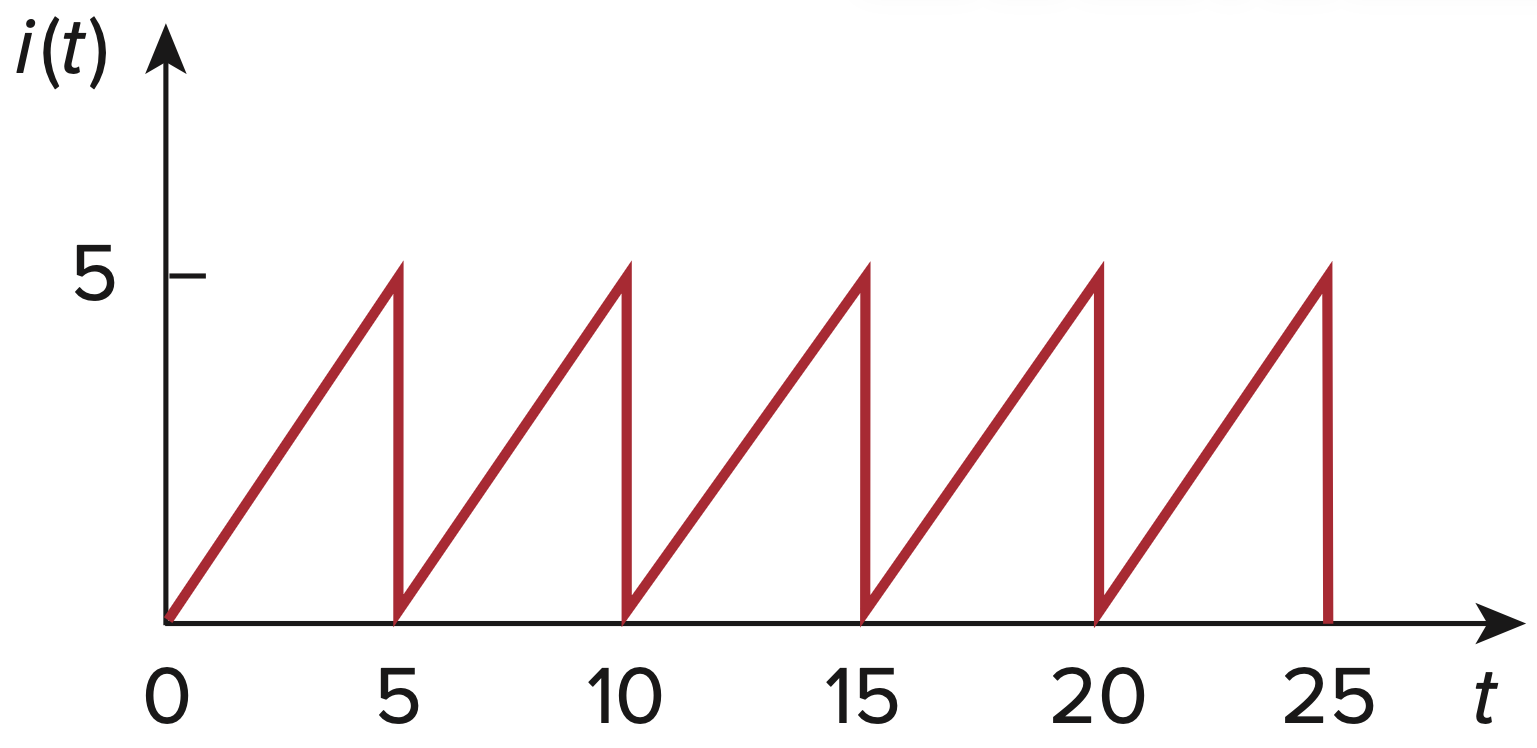
\includegraphics[width=0.7\textwidth]{figures/rms.png}
\end{exercise}

\ifshowsolutions
\begin{solution}
Es handelt sich um eine Sägezahnkurve mit Amplitude 5 A und Periode \(T = 5\,\text{s}\):
\[
I = \sqrt{\frac{1}{T} \int_0^T i^2(t) dt} = \sqrt{\frac{1}{5} \int_0^5 \left(\frac{5t}{5}\right)^2 dt} = \sqrt{\frac{1}{5} \cdot \frac{1}{3} \cdot (5^3 - 0^3)}\,\text{A} \approx 2.89\,\text{A}
\]
\end{solution}
\fi

% ----- Exercise 4 -----
\begin{exercise}[Scheitelwert-Zeiger]
Bestimme die komplexen Amplituden in Bezug auf eine Kosinus-Referenz sowie die kartesische Form der Zeiger für folgende Signale:
\begin{enumerate}[label=\alph*)]
  \item $v(t) = 21 \cos(4t - 15^{\circ})\,\text{V}$
  \item $i(t) = -8 \sin(10t + 70^{\circ})\,\text{mA}$
\end{enumerate}
\end{exercise}

\ifshowsolutions
\begin{solution}
\begin{enumerate}[label=\alph*)]
\item Scheitelwert-Zeiger (Kosinus-Referenz):
\[
\underline{\hat{v}} = 21 \angle -15^{\circ}\,\text{V}
\]
Kartesische Form:
\[
\underline{\hat{v}} = 21 \left(\cos(-15^{\circ}) + j \sin(-15^{\circ})\right)\,\text{V} \approx (20.28 - j5.44)\,\text{V}
\]
\item Umwandlung in Kosinusform:
\[
i(t) = -8 \sin(10t + 70^{\circ})\,\text{mA} = 8 \sin(10t + 250^{\circ})\,\text{mA} = 8 \cos(10t + 160^{\circ})\,\text{mA}
\]
Scheitelwert-Zeiger (Kosinus-Referenz):
\[
\underline{\hat{i}} = 8 \angle 160^{\circ}\,\text{mA}
\]
Kartesische Form:
\[
\underline{\hat{i}} = 8 \left(\cos(160^{\circ}) + j \sin(160^{\circ})\right)\,\text{mA} \approx (-7.52 + j2.74)\,\text{mA}
\]
\end{enumerate}
\end{solution}
\fi

% ----- Exercise 5 -----
\begin{exercise}[Zeiger-Arithmetik]
Zwei Spannungen $v_1$ und $v_2$ sind in Reihe geschaltet, so dass ihre Summe $v = v_1 + v_2$ ist.

Bestimme $v$ für $v_1 = 10\cos(50t - \frac{\pi}{3})\,\text{V}$ und $v_2 = 12\cos(50t + 30^{\circ})\,\text{V}$.
\end{exercise}

\ifshowsolutions
\begin{solution}
Umwandlung beider Spannungen in Zeigerform:
\[
\underline{\hat{v}}_1 = 10 \angle -60^{\circ}\,\text{V}, \quad \underline{\hat{v}}_2 = 12 \angle 30^{\circ}\,\text{V}
\]
Umwandlung in kartesische Form:
\[
\underline{\hat{v}}_1 = 10 \left(\cos(-60^{\circ}) + j \sin(-60^{\circ})\right)\,\text{V} = (5 - j8.66)\,\text{V}
\]
\[
\underline{\hat{v}}_2 = 12 \left(\cos(30^{\circ}) + j \sin(30^{\circ})\right)\,\text{V} = (10.39 + j6)\,\text{V}
\]
Summe der Zeiger:
\[
\underline{\hat{v}} = \underline{\hat{v}}_1 + \underline{\hat{v}}_2 = ((5 + 10.39) + j(-8.66 + 6))\,\text{V} = (15.39 - j2.66)\,\text{V}
\]
Rücktransformation in Polardarstellung:
\[
|\underline{\hat{v}}| = \sqrt{15.39^2 + (-2.66)^2}\,\text{V} \approx 15.62\,\text{V}
\]
\[
\theta = \tan^{-1}\left(\frac{-2.66}{15.39}\right) \approx -9.8^{\circ}
\]
Somit gilt:
\[
\underline{\hat{v}} = 15.62 \angle -9.8^{\circ}\,\text{V}
\]
Rücktransformation in Zeitbereich:
\[
v(t) = 15.62 \cos(50t - 9.8^{\circ})\,\text{V}
\]
\end{solution}
\fi

% ----- Exercise 6 -----
\begin{exercise}[Impedanz]
Eine Reihenschaltung aus Widerstand, Induktivität und Kapazität hat $R = 80\,\Omega$, $L = 240\,\text{mH}$ und $C = 5\,\text{mF}$.

Bestimme den durch die Schaltung fließenden Strom für die Eingangsspannung $v(t) = 10\cos(2t)\,\text{V}$.
\end{exercise}

\ifshowsolutions
\begin{solution}
Kreisfrequenz:
\[
\omega = 2\,\text{rad/s}
\]
Impedanzen der einzelnen Bauelemente:
\[
\underline{Z}_R = 80\,\Omega
\]
\[
\underline{Z}_L = j\omega L = (j2 \cdot 0.24)\,\Omega = j0.48\,\Omega
\]
\[
\underline{Z}_C = \frac{1}{j\omega C} = \frac{1}{j2 \cdot 0.005}\,\Omega = -j100\,\Omega
\]
Totale Impedanz:
\[
\underline{Z} = \underline{Z}_R + \underline{Z}_L + \underline{Z}_C = 80\,\Omega + j0.48\,\Omega - j100\,\Omega = (80 - j99.52)\,\Omega
\]
Betrag und Phase der totalen Impedanz:
\[
|\underline{Z}| = \sqrt{80^2 + (-99.52)^2}\,\Omega \approx 127.69\,\Omega
\]
\[
\theta_Z = \tan^{-1}\left(\frac{-99.52}{80}\right) \approx -51.21^{\circ}
\]
Zeigerform der Spannung:
\[
\underline{\hat{v}} = 10 \angle 0^{\circ}\,\text{V}
\]
Zeigerform des Stroms:
\[
\underline{\hat{i}} = \frac{\underline{\hat{v}}}{\underline{Z}} = \frac{10 \angle 0^{\circ}\,\text{V}}{127.69 \angle -51.21^{\circ}\,\Omega} = \frac{10\,\text{V}}{127.69 \exp(-j51.21^{\circ})\,\Omega} \approx 78.3 \angle 51.21^{\circ}\,\text{mA}
\]
Rücktransformation in Zeitbereich:
\[
i(t) = 78.3 \cos(2t + 51.21^{\circ})\,\text{mA}
\]
\end{solution}
\fi

% ----- Exercise 7 -----
\begin{exercise}[Admittanz]
Bestimme die Admittanz \underline{Y} für die unten dargestellte Schaltung.

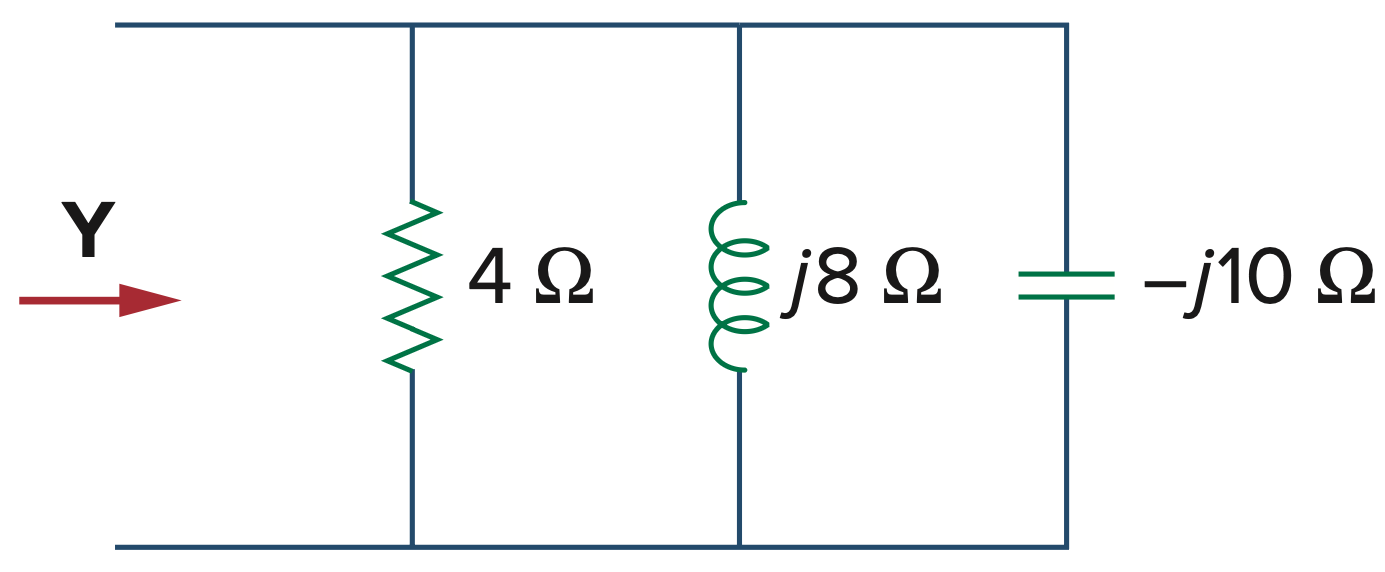
\includegraphics[width=0.7\textwidth]{figures/admittance.png}
\end{exercise}

\ifshowsolutions
\begin{solution}
Berechnung der einzelnen Admittanzen:
\[
\underline{Y}_R = \frac{1}{\underline{Z}_R} = \frac{1}{4\,\Omega} = 0.25\,\text{S}
\]
\[
\underline{Y}_L = \frac{1}{\underline{Z}_L} = \frac{1}{j8\,\Omega} = -j0.125\,\text{S}
\]
\[
\underline{Y}_C = \frac{1}{\underline{Z}_C} = \frac{1}{-j10\,\Omega} = j0.1\,\text{S}
\]
Totale Admittanz:
\[
\underline{Y} = \underline{Y}_R + \underline{Y}_L + \underline{Y}_C = 0.25\,\text{S} - j0.125\,\text{S} + j0.1\,\text{S} = (250 - j25)\,\text{mS}
\]
\end{solution}
\fi

\end{document}